\documentclass[10pt, a4paper]{article}

%%% SST LAB PROTOCOLL PREAMBLE
%%% 2019
%%%%%%%%%%%%%%%%%%%%%%%%%%%%%%%


%%% PACKAGES
%%%%%%%%%%%%%%%%%%%%%%%%%%%

\usepackage[ngerman]{babel}

\usepackage[utf8]{inputenc}
\usepackage{amsmath}
\usepackage{pgfplots}
\usepackage{tikz}
\usepackage[many]{tcolorbox}
\usepackage{graphicx}
\graphicspath{ {./graphics/} }
\usepackage{pdfpages}
\usepackage{dashrule}
\usepackage{float}
\usepackage{siunitx}
\usepackage{trfsigns}
\usepackage{booktabs}
\usepackage[european]{circuitikz}
\usepackage{tcolorbox}

%%% DOCUMENT GEOMETRY
%%%%%%%%%%%%%%%%%%%%%%%%%%%

\usepackage{geometry}
\geometry{
 a4paper,
 total={0.6180339887498948\paperwidth,0.6180339887498948\paperheight},
 top = 0.1458980337503154\paperheight,
 bottom = 0.1458980337503154\paperheight
 }
\setlength{\jot}{0.013155617496424828\paperheight}
\linespread{1.1458980337503154}

\setlength{\parskip}{0.013155617496424828\paperheight} % paragraph spacing


%%% COLORS
%%%%%%%%%%%%%%%%%%%%%%%%%%%

\definecolor{red1}{HTML}{f38181}
\definecolor{yellow1}{HTML}{fce38a}
\definecolor{green1}{HTML}{95e1d3}
\definecolor{blue1}{HTML}{66bfbf}
\definecolor{hsblue}{HTML}{00b1db}
\definecolor{hsgrey}{HTML}{afafaf}

%%% CONSTANTS
%%%%%%%%%%%%%%%%%%%%%%%%%%%
\newlength{\smallvert}
\setlength{\smallvert}{0.0131556\paperheight}


%%% COMMANDS
%%%%%%%%%%%%%%%%%%%%%%%%%%%

% differential d
\newcommand*\dif{\mathop{}\!\mathrm{d}}

% horizontal line
\newcommand{\holine}[1]{
  	\begin{center}
	  	\noindent{\color{hsgrey}\hdashrule[0ex]{#1}{1pt}{3mm}}\\%[0.0131556\paperheight]
  	\end{center}
}

% mini section
\newcommand{\minisec}[1]{ \noindent\underline{\textit {#1} } \\}

% quick function plot
\newcommand{\plotfun}[3]{
  \vspace{0.021286\paperheight}
  \begin{center}
    \begin{tikzpicture}
      \begin{axis}[
        axis x line=center,
        axis y line=center,
        ]
        \addplot[draw=red1][domain=#2:#3]{#1};
      \end{axis}
    \end{tikzpicture}
  \end{center}
}

% box for notes
\newcommand{\notebox}[1]{

\tcbset{colback=white,colframe=green1!100!black,title=Note!,width=0.618\paperwidth,arc=0pt}

 \begin{center}
  \begin{tcolorbox}[]
   #1 
  \end{tcolorbox}
 
 \end{center} 
 
}

% box for equation
\newcommand{\eqbox}[2]{
	
	\tcbset{colback=white,colframe=green1!100!black,title=,width=#2,arc=0pt}
	
	\begin{center}
		\begin{tcolorbox}[ams align*]
				#1
		\end{tcolorbox}
		
	\end{center} 
	
}
% END OF PREAMBLE
\renewcommand{\thempfootnote}{\arabic{mpfootnote}}

\begin{document}


\includepdf{./titlepage/titlepage.pdf}

\section*{Homework Tasks}
\begin{taskspec}

HW5)\\

due May 25th 23:59 LT\\

1)\\
- familiarize with antennas and antenna types (textbooks, wiki etc.)\\

2)\\
categorize and briefly summarize antenna types and their properties (gain, beam width, band width, impedance, characteristic sizes)\\

- single antennas: (nearly) omni-directional, directional (yagi, patch, parabolic dish)\\

- antenna groups (co-linear, antenna arrays)\\

include examples of corresponding radiation pattern\\
\end{taskspec}

\pagebreak

\section{Some Definitions}
%The following short definitions regarding antennas have been compiled using x and y \todo{cite a b}.

\begin{description}
\item[Antenna] A device which translates guided electromagnetic waves on a transmission line to waves in free space (and vice versa).
\item[Radiation Pattern $F$] The distribution of power (intensity) radiated from an antenna as a function of direction, in spherical coordinates (azimuth $\phi$, elevation $\theta$). Usually normalized to its maximum value.
\item[Directivity $D$] The power density as a function of direction normalized to the average power density of all directions. Antenna specifications typically give the directivity as peak directivity for all directions. It will determine how much more power the antenna radiates in its peak direction compared to an isotropic reference antenna.
\item[Gain $G$] Is similar to the directivity in that it describes the power density in the preak direction with reference to that of an isotropic antenna but it also takes into account losses. Especially relevant with electrically short antennas.
\item[Beamwidth] For directional antennas, the angle from the peak of the main lobe of the radiation pattern to the point at which the radiated power density decreases by a specified factor, typically $50\,\si{\percent}$ or $-3\,\si{\deci\bel}$ (Half Power Beam Width, HPBW).
\item[(Feedpoint-)Impedance] The relationship between the voltage and current at the input of the antenna (complex number). Typically for resonant antennas, the reactive part should be close to zero and the impedance should stay constant in the desired frequency band and matched to the feeding transmitter to allow for a low reflection coefficient.
\item[Polarization] Direction of the electric (and magnetic) field oscillation over time. If it stays constant, the field is said to be linearly polarized. The direction can also change if the electric field can be decomposed into components that are out of phase by $90\,\si{\degree}$. If the amplitude of these components is the same, the field is called cirularly polarized. If it is different, it is called eliptically polarized.
\item[Antenna Arrays] A collection of antennas that forms a combined radiation pattern. Often, the antennas can be driven individually to provide each with a different phase angle.
\end{description}



\pagebreak
\section{Antenna Types}

The following table \ref{tab:ant1} shows a few antenna examples with characteristic numbers.
Some radiation patterns for can also be seen in the figures below. Most of these characteristics are dependent upon the antenna geometry and are therefore only rough typical values.\\


\begin{table}[h]

\centering

\begin{minipage}{\textwidth}
\begin{tabular}{lcccccc} \toprule
    {Name} & {$D$ ($\si{\deci\bel}$)} & {$3\,\si{\deci\bel}$-Beamw.} & {Impedance} & {Bandwidth} & {Polarization} & {Typical Sizes} \\ \midrule\midrule
  {(nearly) omni-dir.} & & & & & & \\
  \midrule
    {$\lambda/2$ Dipole}  & 2.15 & $\approx 80\,\si{\degree}$ & $73\,\si{\ohm}$ & narrow & linear & $\lambda/2$  \\
  {$\lambda/4$ Monopole}  & 5.2  & $\approx 40\,\si{\degree}$ & $36.5\,\si{\ohm}$ & narrow & linear & $\lambda/4$ \\
  \midrule
  {directional} & & & & & & \\
  \midrule
    {Patch}  & 5{...}8  & typ. $65\,\si{\degree}$ & $50..300\,\si{\ohm}$ \footnote{depends on patch width}  & narrow & linear & some $10 \,\si{\milli\meter}$\\
    {Helix (Axial-Mode)}  & 8...14 & $\frac{5}{2}\frac{C}{\lambda}\sqrt{\frac{N\cdot S}{\lambda}}$  \footnote{$C$: circumference of one turn, $N$: number of turns, $S$: axial pitch between turns}  & $\approx 140\cdot C / \lambda$  & narrow & elliptical & $50\,\si{\milli\meter}$...few $\si{\meter}$\\
    {Horn}  & 10{...}20  & $11\,\si{\degree}...15\,\si{\degree}$  & $50\,\si{\ohm}$ \footnote{can be matched to waveguide geometry}  & wide & linear & $50...400\,\si{\mm}$ \\
    {Yagi}  & {...}20  & $30\,\si{\degree}...70\,\si{\degree}$ & $10...40\,\si{\ohm}$  & narrow & linear & $<10\,\si{\meter}$ \\
    {Parabolic}  & 10{...}40  & $\approx 70\lambda / D\,\si{\degree}$ \footnote{$D$ is the aperture diameter} & depends \footnote{depends on feed antenna}  & wide & depends \footnote{depends on feed antenna}  & $0.5...500\,\si{\meter}$ \footnote{see FAST radio telescope} \\ \midrule
  {antenna groups} & & & & & & \\
  \midrule
    {2x2 Patch Array}  & > patch  & $\approx 15\,\si{\degree}$ & $50\,\si{\ohm}$ & narrow  & linear &  some $10\,\si{\milli\meter}$\\
    {Collinear Dipoles}  & $10\cdot\log{n}$ \footnote{$n:$ number of elements, gain relative to single element}  & $\propto 1/n$ & $73\,\si{\ohm} / n$ & narrow & linear & $n \cdot (\lambda / 2 + s)$ \\
    \bottomrule
\end{tabular}
\end{minipage}

\caption{Compilation of different antenna types.}\label{tab:ant1}

\end{table}

% https://en.wikipedia.org/wiki/Parabolic_antenna
% https://en.wikipedia.org/wiki/Collinear_antenna_array
% https://en.wikipedia.org/wiki/Monopole_antenna


\begin{table}[h]

\centering

\begin{minipage}{\textwidth}
  \centering
\begin{tabular}{p{0.15\linewidth}p{0.6\linewidth}} \toprule
    {Name} & Typical Uses\\ \midrule\midrule
    Dipole & fixed-frequency, omnidirectional applicatins, e.g. WiFi routers \\ \midrule
    Monopole & mobile devices, vehicles\\ \midrule
    Patch & PCBs and ICs\\ \midrule
    Helix & where circular polarization is needed, e.g. certain space communication\\ \midrule
    Horn & waveguides, feed for parabolic antennas, low-loss applications\\\midrule
    Yagi & terrestrial communication, fixed-frequency applications \\\midrule
    Parabolic & satellite communication links, radio telescopes\\\midrule
    Arrays & interferometry, beamsteering applications\\
    \bottomrule
\end{tabular}
\end{minipage}

\caption{Typical antenna application areas.}\label{tab:ant2}

\end{table}

% https://en.wikipedia.org/wiki/Parabolic_antenna
% https://en.wikipedia.org/wiki/Collinear_antenna_array
% https://en.wikipedia.org/wiki/Monopole_antenna


\begin{figure}[H]
  \begin{minipage}[t]{0.45\textwidth}
    \centering
    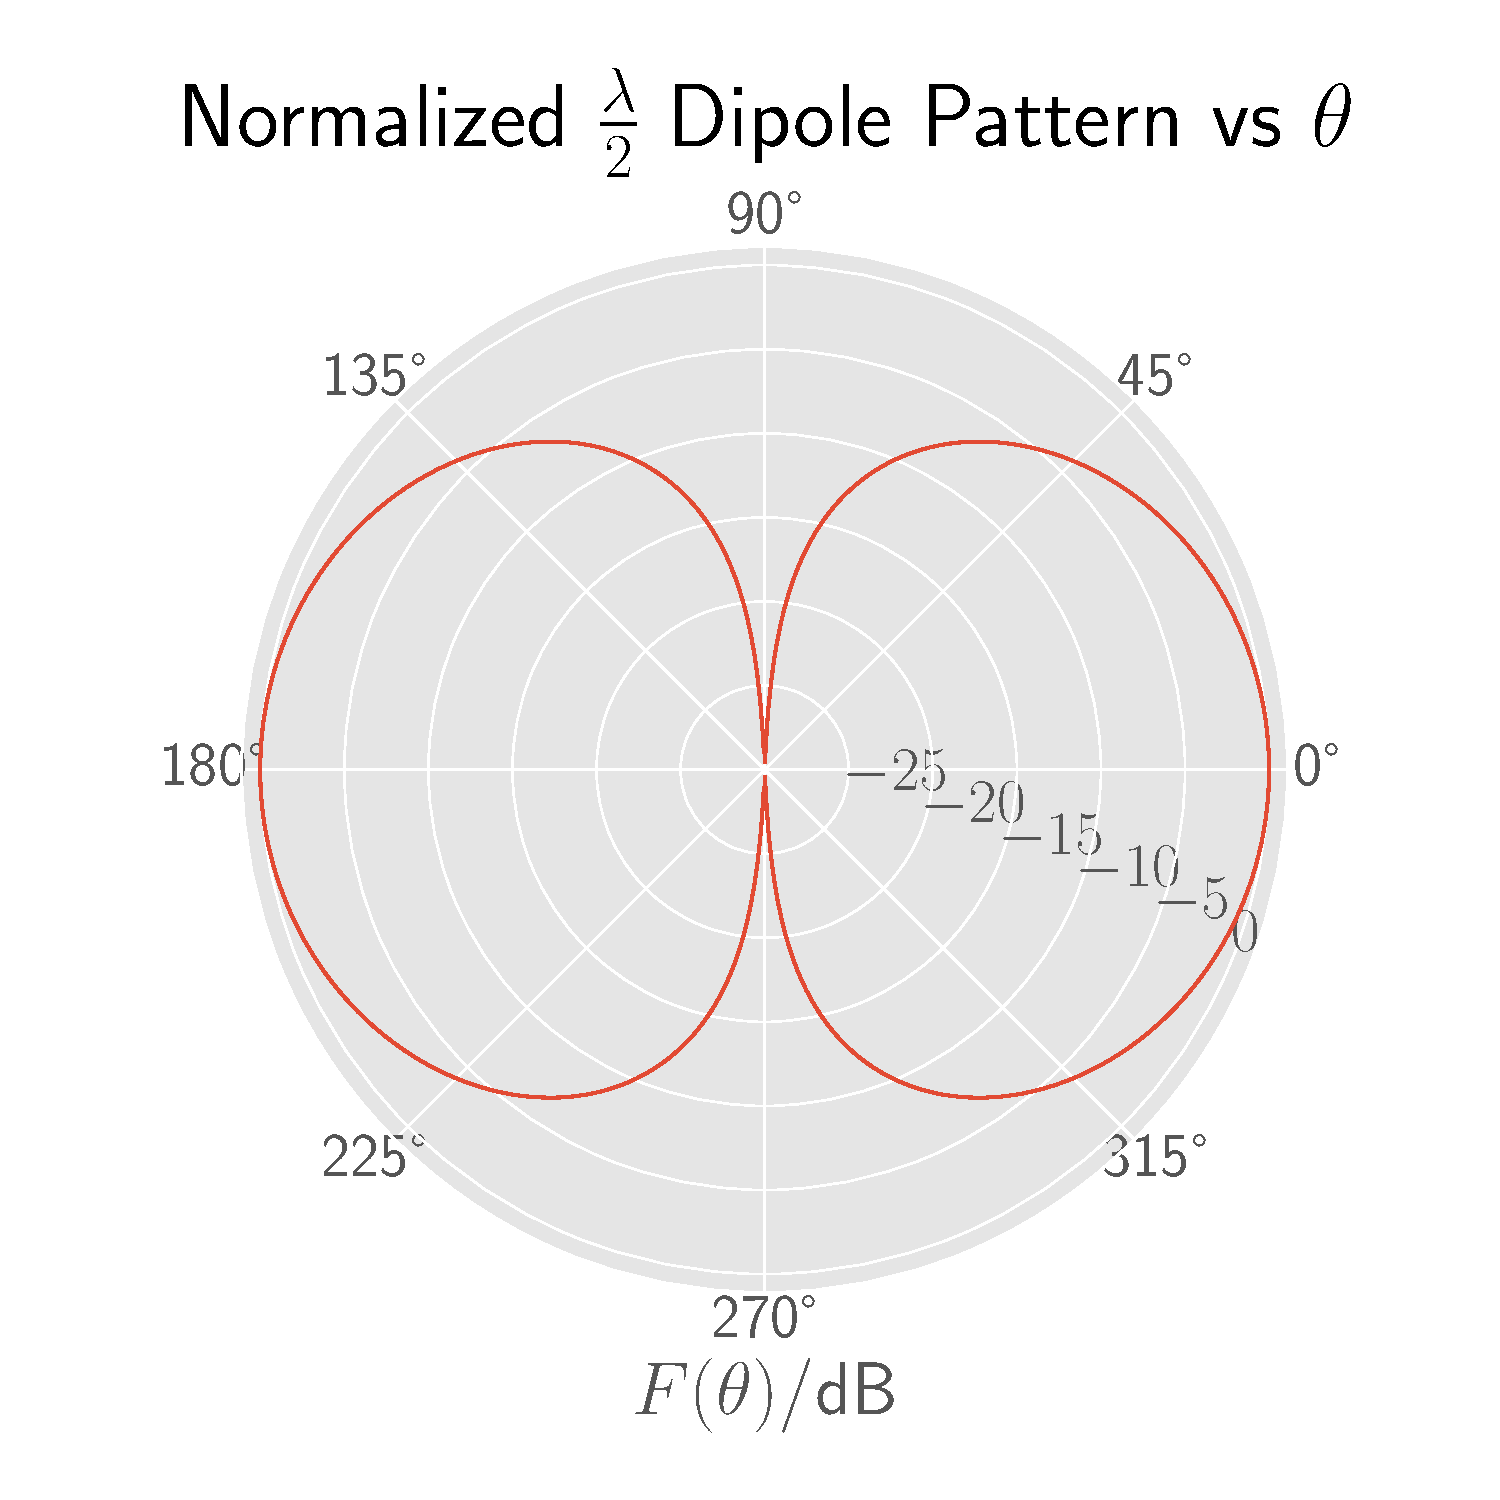
\includegraphics[width=\textwidth]{graphics/dipole_theta.pdf}
    \caption{$\lambda/4$ Dipole characteristic in the elevation plane. Antenna axis lies vertically.}
  \end{minipage}\hfill
  \begin{minipage}[t]{0.45\textwidth}
    \centering
    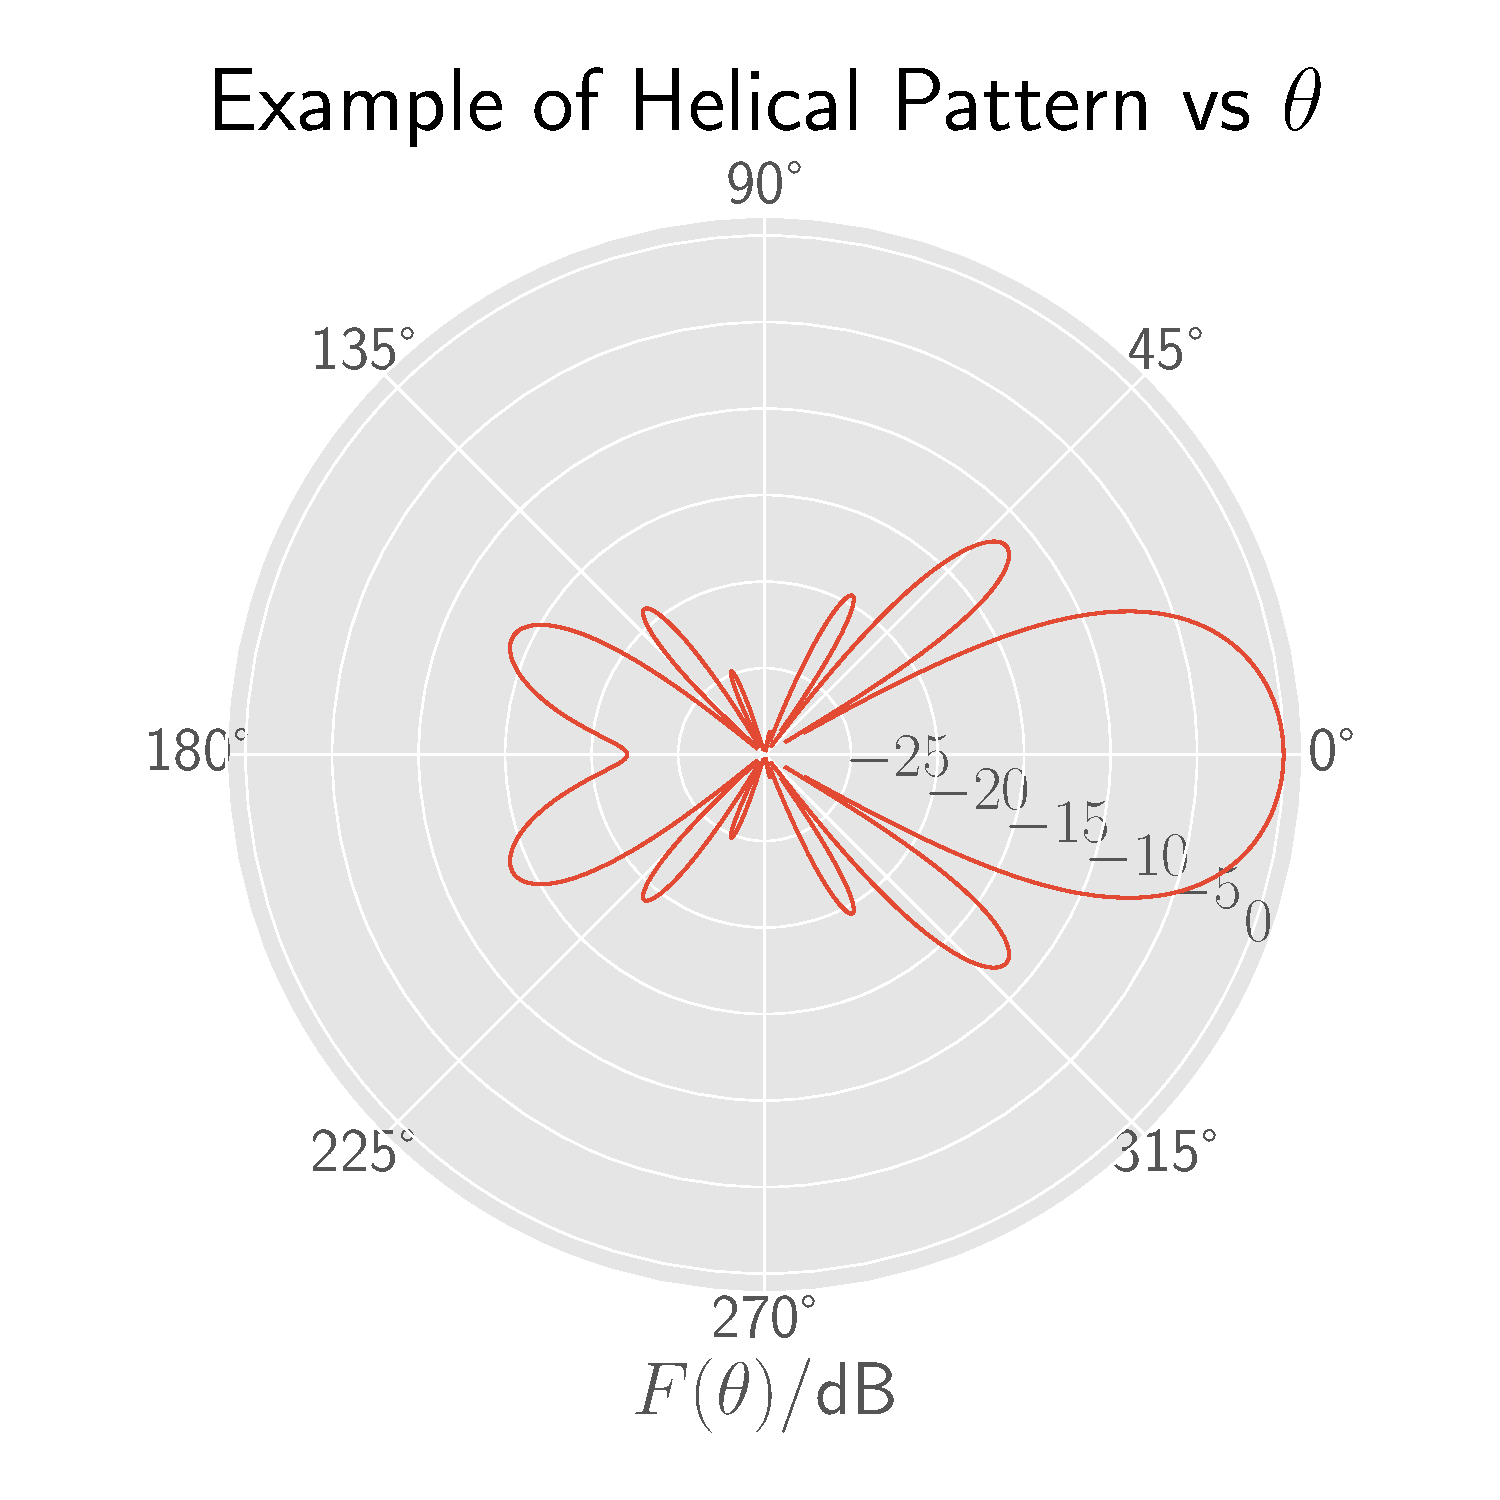
\includegraphics[width=\textwidth]{graphics/helical_theta.pdf}
    \caption{Helical characteristic in the elevation plane. Separation: $0.22\,\si{\meter}$, Number of turns: $10$, Frequency: $500\,\si{\mega\hertz}$ ($\lambda=0.6\,\si{\meter}$)}
  \end{minipage}
\end{figure}



\begin{figure}[H]
  \begin{minipage}[t]{0.45\textwidth}
    \centering
    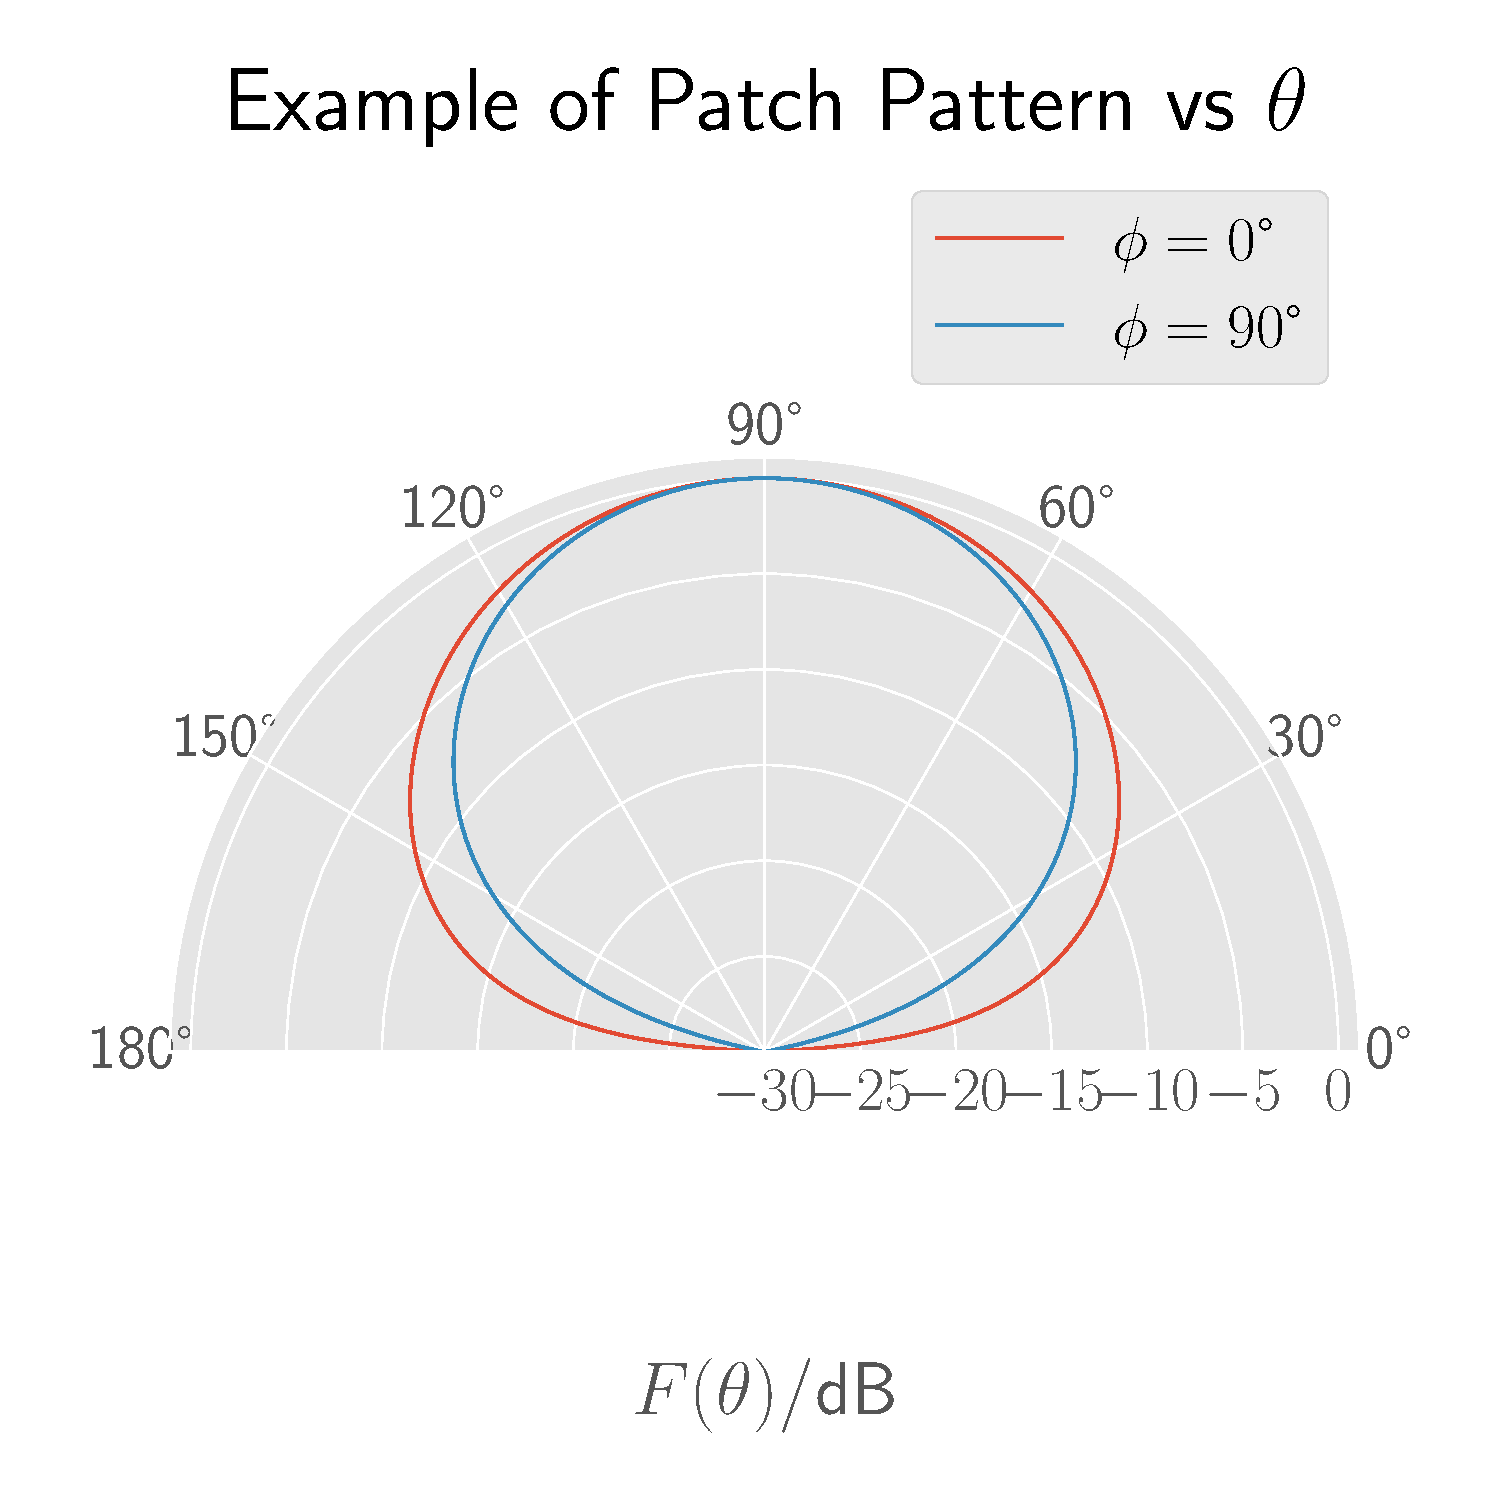
\includegraphics[width=\textwidth]{graphics/patch_theta.pdf}
    \caption{Single Patch characteristic in the elevation plane for two different $\phi$ angles. $W=L=0.5\,\si{\lambda}$.}
  \end{minipage}\hfill
  \begin{minipage}[t]{0.45\textwidth}
    \centering
    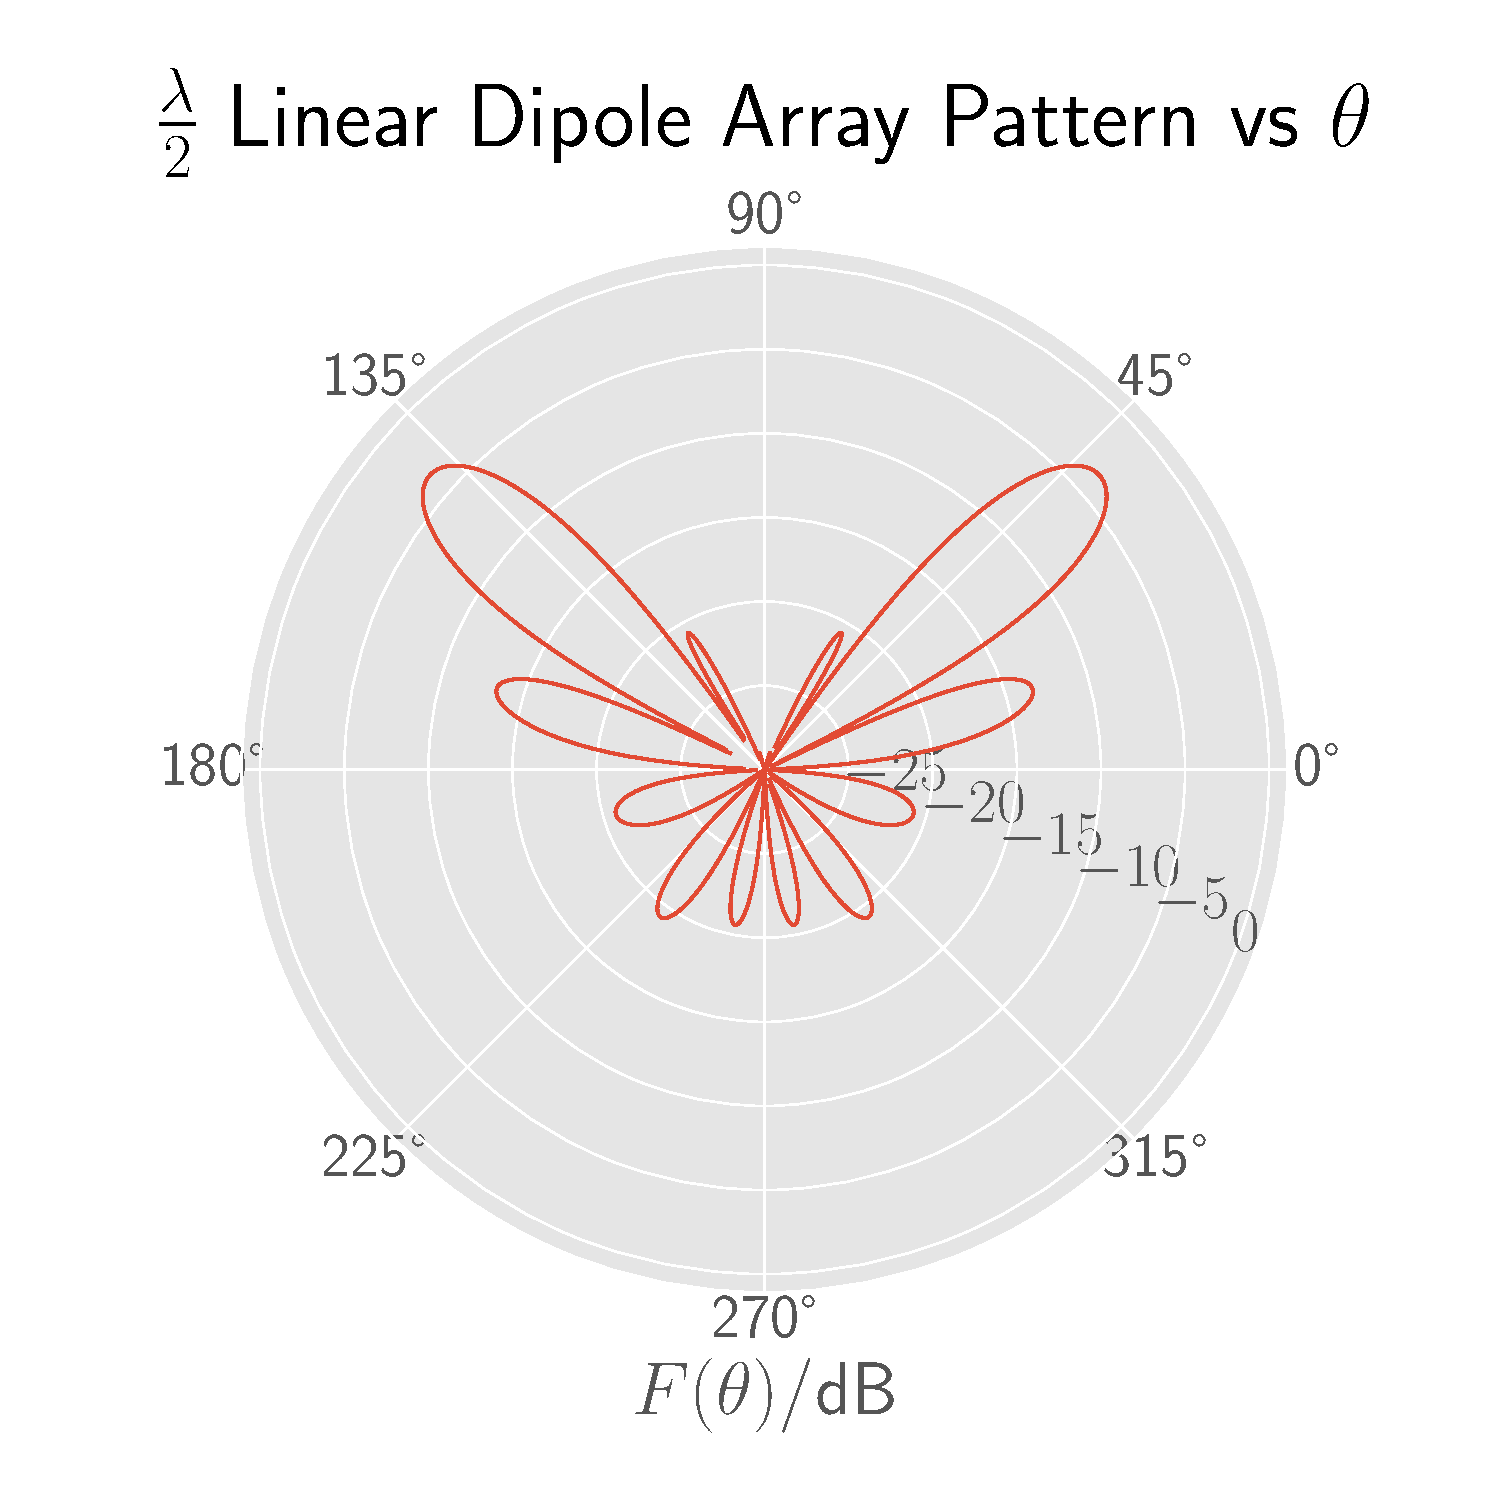
\includegraphics[width=\textwidth]{graphics/dipole_array_theta.pdf}
    \caption{Characteristic of equally spaced linear dipole array in the elevation plane. $N=8$, Separation: $\lambda/2$}
  \end{minipage}
\end{figure}


\begin{figure}[H]
  \begin{minipage}[t]{0.45\textwidth}
 \centering
  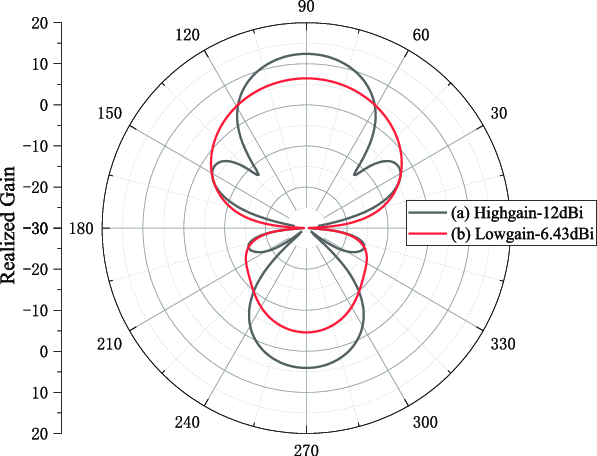
\includegraphics[width=\textwidth]{graphics/yagi.png}
  \caption{Example of a Yagi-Uda characterisitic. Taken from \url{https://www.researchgate.net/figure/Radiation-patterns-of-two-Yagi-Uda-antennas-a-with-high-gain-and-b-with-low-gain_fig2_363745716} under CC BY-NC-ND 4.0}

  \end{minipage}\hfill
  \begin{minipage}[t]{0.45\textwidth}
  \centering
  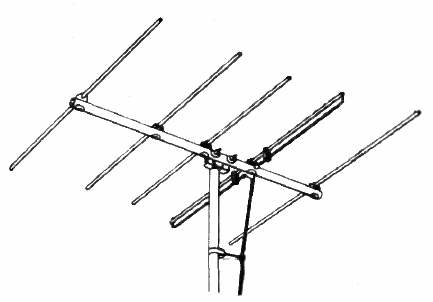
\includegraphics[width=\textwidth]{graphics/yagi2.png}
  \caption{Drawing of a typical Yagi-Uda antenna.}
  \end{minipage}
\end{figure}


\begin{figure}[H]
  \begin{minipage}[t]{0.45\textwidth}
    \centering
    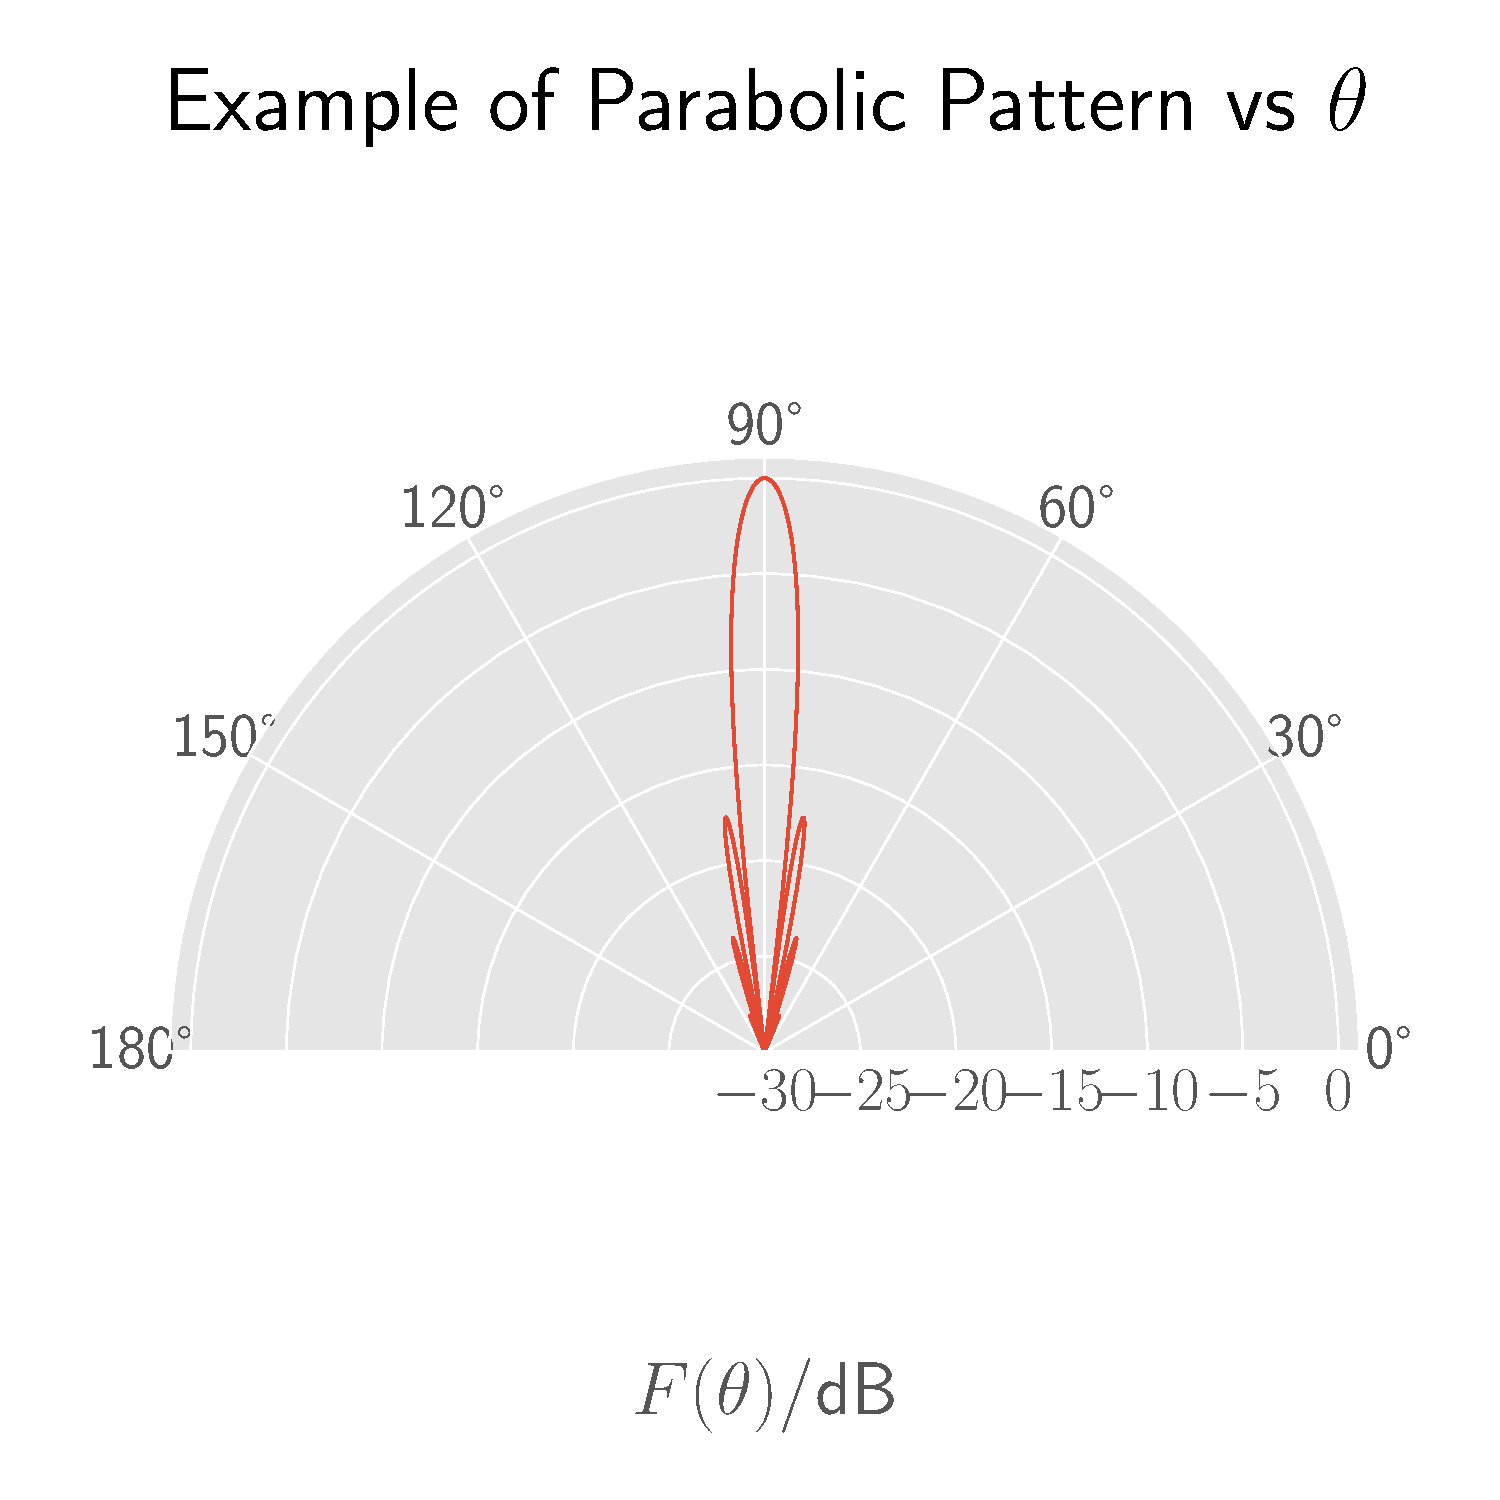
\includegraphics[width=\textwidth]{graphics/parabolic_theta.pdf}
    \caption{Example of Parabolic characteristic for $D=10\lambda$.}
  \end{minipage}\hfill
  \begin{minipage}[t]{0.45\textwidth}
    \centering
    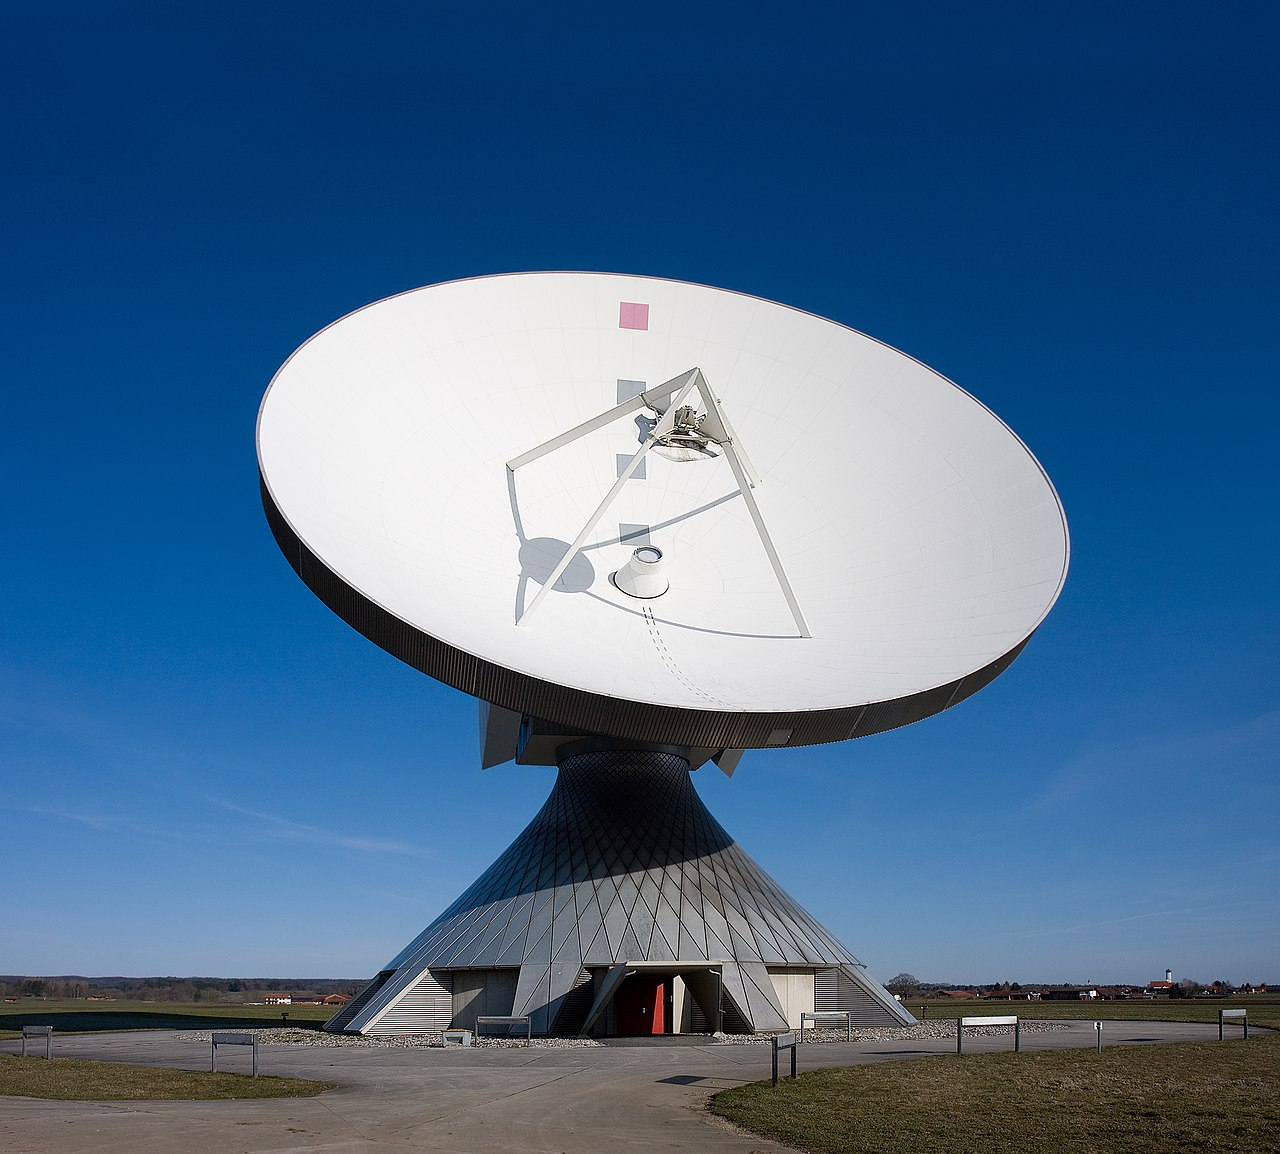
\includegraphics[width=\textwidth]{graphics/parab.jpg}
    \caption{Satellite communications parabolic antenna. Taken from \url{https://en.wikipedia.org/wiki/Parabolic_antenna\#/media/File:Erdfunkstelle_Raisting_2.jpg} under CC BY-SA 2.5}
   \end{minipage}
\end{figure}



% ------------------------------------------------------------------------------

\printbibheading
\begin{refsection}[sources.bib]
\nocite{*}
\printbibliography[heading=subbibliography,title={Literature}]
\end{refsection}

\begin{refsection}[web.bib]
\nocite{*}
\printbibliography[heading=subbibliography,title={Web}]
\end{refsection}

% \begin{refsection}[software.bib]
% \nocite{*}
% \printbibliography[heading=subbibliography,title={Software Used}]
% \end{refsection}

\end{document}
